\section{Design}
\label{sec:design}
Around 5 pages about functional aspects of the FeedApp application.
Concretely, you shall write about 
\begin{itemize}
	\item the \emph{use cases},
	\item the \emph{domain model}, and
	\item the \emph{architecture} (including applied technologies)
\end{itemize}
Each part shall ideally be accompanied with a graphical representation (diagram).
You may have a look at the \href{https://github.com/selabhvl/dat250public/blob/master/projectdescription/README.md}{Examples on GitHub}.
In this section, we provide an overview of the functional aspects of the FeedApp application, focusing on the use cases, domain model, and architecture, including the technologies used in the backend, frontend, and messaging layers.
\begin{itemize}
    \item Source: \href{https://chatgpt.com/share/672fbc4f-ecf4-8007-b147-6759b1884b9c}{ChatGPT}
\end{itemize}
\subsection{Use Cases}
The FeedApp application provides a polling system where users can create, participate in, and manage polls. The key use cases are as follows:
\begin{itemize}
    \item \textbf{User Registration and Authentication:} Users can create an account, log in, and authenticate via email and password. This ensures that only registered users can create and vote in polls.
    \item \textbf{Poll Creation:} Authenticated users can create new polls by submitting a question and providing multiple voting options. Only registered users can create polls.
    \item \textbf{Vote on Polls:} Registered users can vote on available polls by selecting one of the options. Each user can vote only once per poll.
    \item \textbf{View Poll Results:} Users can view the current results of active polls, including the vote counts for each option.
    \item \textbf{Edit and Delete Polls:} Poll creators can edit or delete polls they have created, provided the poll is still open.
    \item \textbf{Vote Modification:} Users can modify their vote in an active poll.
    \item \textbf{Event Logging:} The system logs key events, such as vote casting, poll creation, and poll editing, for auditing and analytics purposes.
\end{itemize}
Each use case is supported by the backend services to ensure proper functionality, and the user interface provides a seamless experience for interacting with these actions.
\subsection{Domain Model}
The domain model of the FeedApp consists of several key entities that represent the core data objects of the system. These entities are mapped to the database and interact through the business logic.
\begin{itemize}
    \item \textbf{User:} Represents the users of the system. Each user has a unique identifier, email, password, and roles (admin, voter).
    \item \textbf{Poll:} Represents a poll created by a user. A poll has a unique identifier, a question, multiple options for voting, and a status (active, closed).
    \item \textbf{Vote:} Represents a vote cast by a user on a specific poll. A vote has a reference to the user who cast it, the poll being voted on, and the selected option.
    \item \textbf{Event:} Represents events logged in the system, such as vote events, poll creation events, and poll edit events. Events are tracked for auditing and analytics purposes.
\end{itemize}
The diagram above illustrates the relationships between the entities, with associations such as a user creating a poll, casting a vote, and generating events.
\subsection{Architecture and Applied Technologies}
The architecture of the FeedApp is designed to be modular and scalable, with separate services responsible for managing user data, polls, votes, and events. 
\begin{itemize}
    \item \textbf{Backend Framework and Language:} 
    \begin{itemize}
        \item \textbf{Spring Boot:} Used for building the backend API, providing RESTful endpoints for managing users, polls, and votes.
        \item \textbf{Kotlin:} Chosen for its concise syntax and interoperability with Java, making it a great fit for Spring Boot applications.
    \end{itemize}
    
    \item \textbf{Persistence Layer:} 
    \begin{itemize}
        \item \textbf{Spring JPA:} Used for database access with ORM (Object-Relational Mapping) support. Polls and votes are stored in PostgreSQL, while MongoDB is used for logging events.
        \item \textbf{PostgreSQL:} Relational database used to store user and poll data.
        \item \textbf{MongoDB:} Non-relational database used for storing event logs, providing scalability and flexibility for log data.
    \end{itemize}
    
    \item \textbf{Frontend Framework:} 
    \begin{itemize}
        \item \textbf{SvelteKit:} A modern frontend framework used for building fast, reactive web applications with minimal overhead.
    \end{itemize}
    
    \item \textbf{Messaging:}
    \begin{itemize}
        \item \textbf{RabbitMQ:} Used as a message broker to handle asynchronous communication between services. Events like votes and poll updates are sent to RabbitMQ for processing and tracking.
    \end{itemize}
    \item \textbf{Containerization and Deployment:} 
    \begin{itemize}
        \item \textbf{Docker:} The entire application, including the backend, frontend, and database, is containerized using Docker for easy deployment and scalability.
    \end{itemize}
\end{itemize}
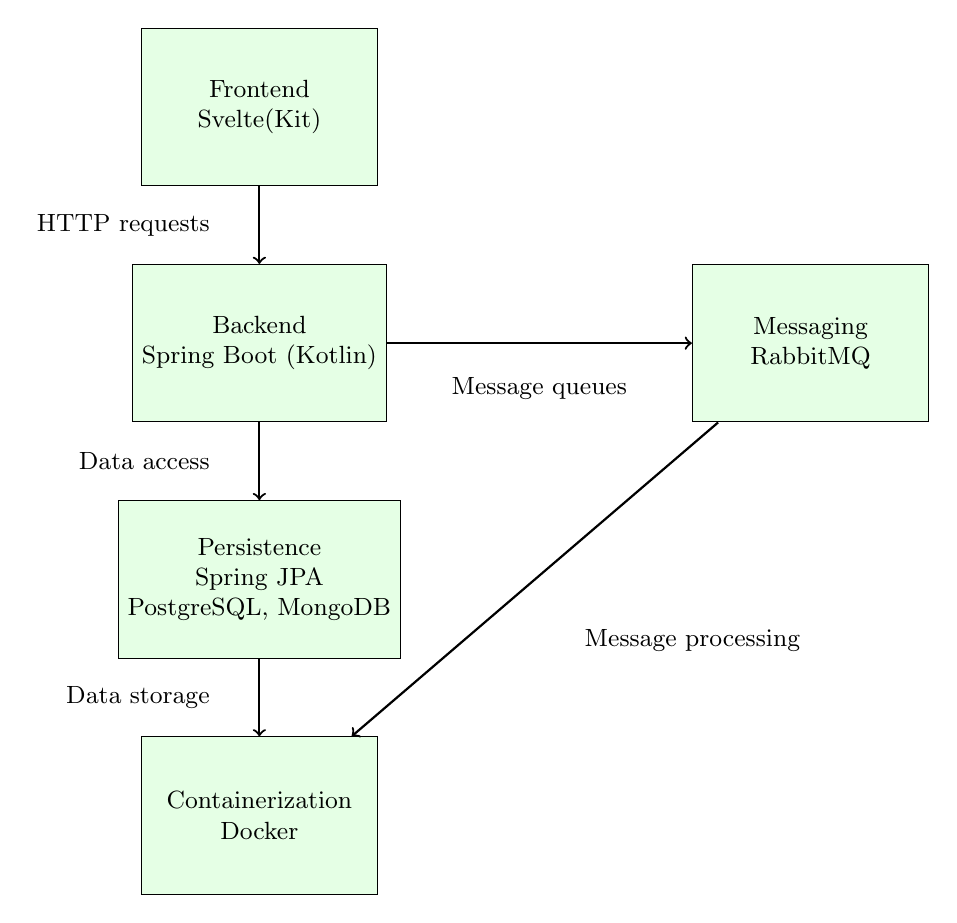
\begin{tikzpicture}[node distance=3cm, auto, font=\small]
    % Define the blocks for each component
    \node (frontend) [draw, rectangle, fill=green!10, text centered, minimum height=2cm, minimum width=3cm, align=center] {Frontend \\ Svelte(Kit)};
    \node (backend) [draw, rectangle, fill=green!10, below of=frontend, text centered, minimum height=2cm, minimum width=3cm, align=center] {Backend \\ Spring Boot (Kotlin)};
    \node (persistence) [draw, rectangle, fill=green!10, below of=backend, text centered, minimum height=2cm, minimum width=3cm, align=center] {Persistence \\ Spring JPA \\ PostgreSQL, MongoDB};
    \node (messaging) [draw, rectangle, fill=green!10, right of=backend, xshift=4cm, text centered, minimum height=2cm, minimum width=3cm, align=center] {Messaging \\ RabbitMQ};
    \node (container) [draw, rectangle, fill=green!10, below of=persistence, text centered, minimum height=2cm, minimum width=3cm, align=center] {Containerization \\ Docker};
    % Draw arrows to show the flow of interaction
    \draw[->, thick] (frontend) -- (backend) node[midway, left, xshift=-0.5cm] {HTTP requests};
    \draw[->, thick] (backend) -- (persistence) node[midway, left, xshift=-0.5cm] {Data access};
    \draw[->, thick] (backend) -- (messaging) node[midway, below, yshift=-0.3cm] {Message queues};
    \draw[->, thick] (persistence) -- (container) node[midway, left, xshift=-0.5cm] {Data storage};
    \draw[->, thick] (messaging) -- (container) node[midway, below, yshift=-0.5cm, xshift=2cm] {Message processing};
\end{tikzpicture}
\subsection{Backend}
We will now look into how the Kotlin code is organized. We use Kotlin with Spring Boot as the backend. The code is organized into three main services: EventService, PollService, and UserService. These handle the business logic. We also have class JwtService,  which provides token management for authentication.
 
\vspace{1cm}
\vspace{1cm}
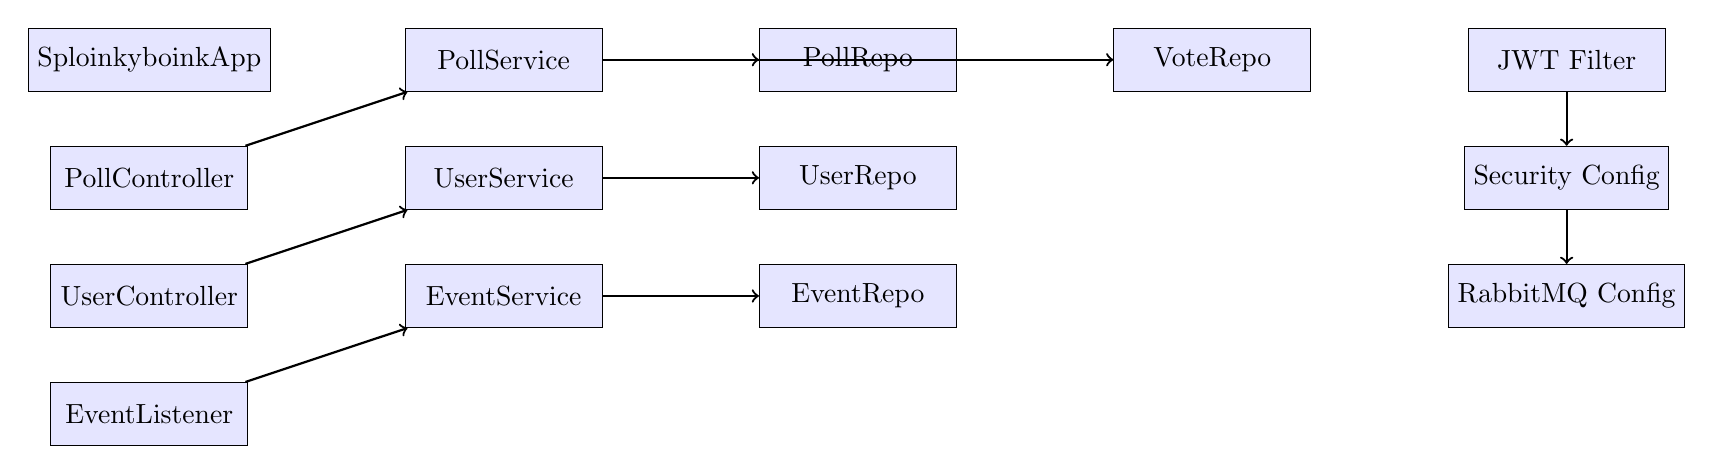
\begin{tikzpicture}[node distance=1.5cm]
% Define UML class styles
\tikzstyle{class} = [rectangle, draw=black, fill=blue!10, text centered, minimum height=0.8cm, minimum width=2.5cm]
\tikzstyle{arrow} = [->, thick, draw=black]
% Define nodes (classes)
\node[class] (SploinkyboinkApplication) {SploinkyboinkApp};
\node[class, below of=SploinkyboinkApplication] (PollController) {PollController};
\node[class, below of=PollController] (UserController) {UserController};
\node[class, below of=UserController] (EventListener) {EventListener};
% Define second layer nodes (Services)
\node[class, right of=SploinkyboinkApplication, xshift=3cm] (PollService) {PollService};
\node[class, below of=PollService] (UserService) {UserService};
\node[class, below of=UserService] (EventService) {EventService};
% Define third layer nodes (Repositories)
\node[class, right of=PollService, xshift=3cm] (PollRepository) {PollRepo};
\node[class, below of=PollRepository] (UserRepository) {UserRepo};
\node[class, below of=UserRepository] (EventRepository) {EventRepo};
\node[class, right of=PollRepository, xshift=3cm] (VoteRepository) {VoteRepo};
% Define fourth layer nodes (Security)
\node[class, right of=VoteRepository, xshift=3cm] (JwtAuthFilter) {JWT Filter};
\node[class, below of=JwtAuthFilter] (SecurityConfig) {Security Config};
% Define fifth layer nodes (Configurations)
\node[class, below of=SecurityConfig] (RabbitMQConfig) {RabbitMQ Config};
% Relationships (arrows)
\draw[arrow] (PollController) -- (PollService);
\draw[arrow] (UserController) -- (UserService);
\draw[arrow] (EventListener) -- (EventService);
\draw[arrow] (PollService) -- (PollRepository);
\draw[arrow] (PollService) -- (VoteRepository);
\draw[arrow] (UserService) -- (UserRepository);
\draw[arrow] (EventService) -- (EventRepository);
\draw[arrow] (JwtAuthFilter) -- (SecurityConfig);
\draw[arrow] (SecurityConfig) -- (RabbitMQConfig);
\end{tikzpicture}
\vspace{1cm}
\begin{itemize}
    \item \textbf{EventService}: Manages event logging, such as user votes and poll creation/editing.
    \item \textbf{PollService}: Handles poll management and voting logic.
    \item \textbf{UserService}: Manages user registration, authentication, and user data operations.
    \item \textbf{JwtService}: Provides token management for authentication.
    \item \textbf{Repositories}:The application uses repositories for data access (\texttt{PollRepo}, \texttt{UserRepo}, \texttt{VoteRepo}, \texttt{EventRepo}) and includes JWT filters for security, with RabbitMQ configured for message handling.
\end{itemize}
\vspace{0.5cm}
\textbf{Achieved functionalities}
\begin{itemize}
    \item \textbf{Polling Functionality}: Users can create, manage, and participate in polls, with their votes accurately captured and stored.
    \item \textbf{Event Tracking}: Tracks important user actions, enabling auditing or analytics.
    \item \textbf{User Management}: Ensures secure user authentication and management through validation mechanisms.
    \item \textbf{Integration with Messaging}: RabbitMQ integration supports a scalable, event-driven architecture, enabling the decoupling of services and enhancing overall application performance.
\end{itemize}